%describe the background necessary to understand the lab's content, with some reservation (i.e., not too much detail)
%possibly provide walkthrough for simple problem
\section{Introduction}

In this lab you will be creating a chromatic tuner, which is a device that tells a user what musical note is closest to the one being played into the tuner's microphone.
In order to accomplish this on Android, you must utilize its onboard microphone and directly analyze the incoming audio data.
Aiding you in this task is a function called the \ac{fft}.

The \ac{fft} is a special case of the more general Fourier transform in that the \ac{fft} only applies to discrete data.
The \ac{fft} has various applications, but the application for which it will be used here is to decompose an audio waveform into its constituent frequencies.
A full discussion of the Fourier transform is beyond the scope of this lab and this course, but some examples of it in action will be given.
Please note that these examples are meant to illustrate concepts rather than be perfectly accurate in their results.
Figure~\ref{fig:cft} demonstrates the result of a continuous Fourier transform applied upon a sine wave.
\begin{figure}[h]
\centering
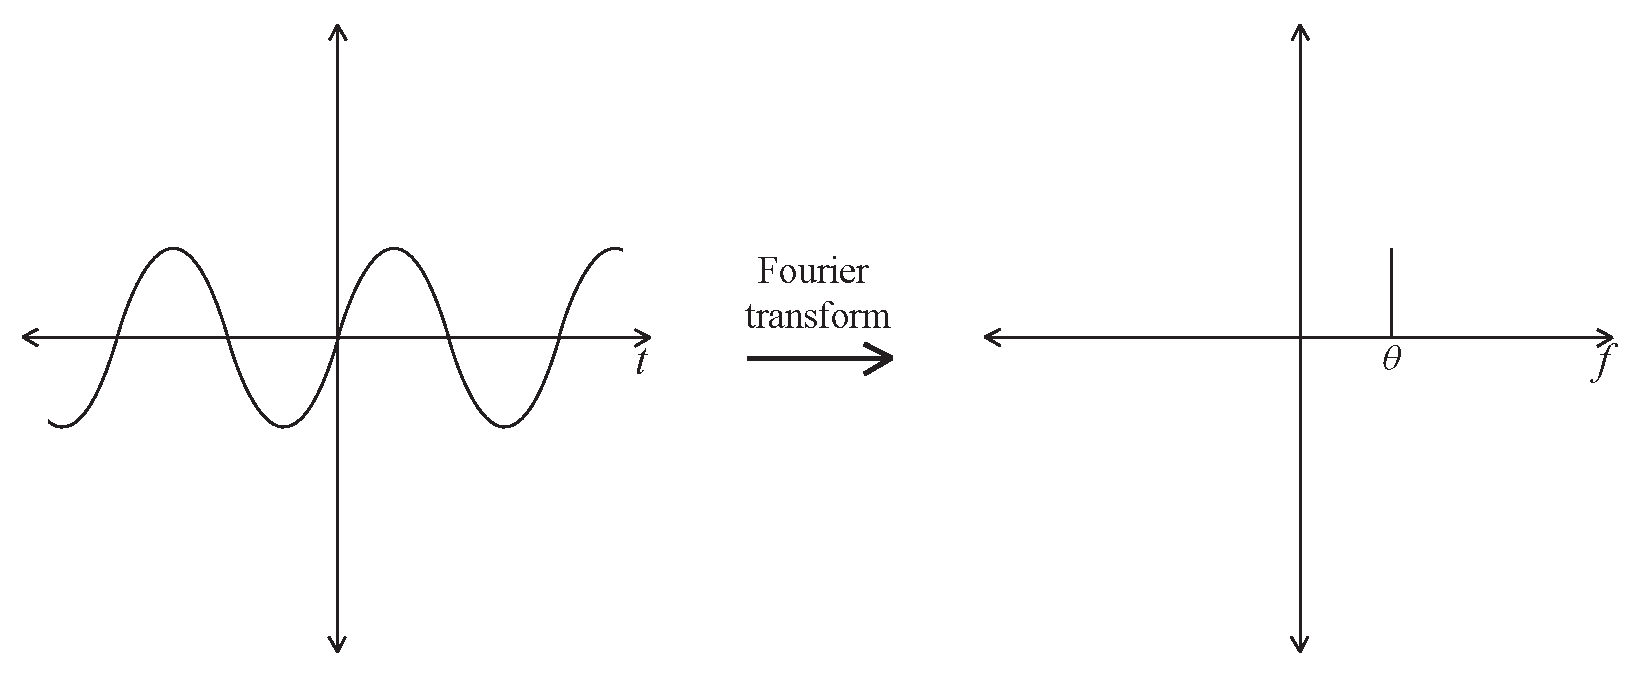
\includegraphics[width=0.8\textwidth]{CFT.pdf}
\caption{The Fourier transform of a sine wave with frequency $\theta$ in the time domain results in a single peak in the frequency domain at $\theta$.}
\label{fig:cft}
\end{figure}
Figure~\ref{fig:dft} on the other hand illustrates the expected results of a discrete Fourier transform applied upon a discretized sine wave.
\begin{figure}[h]
\centering
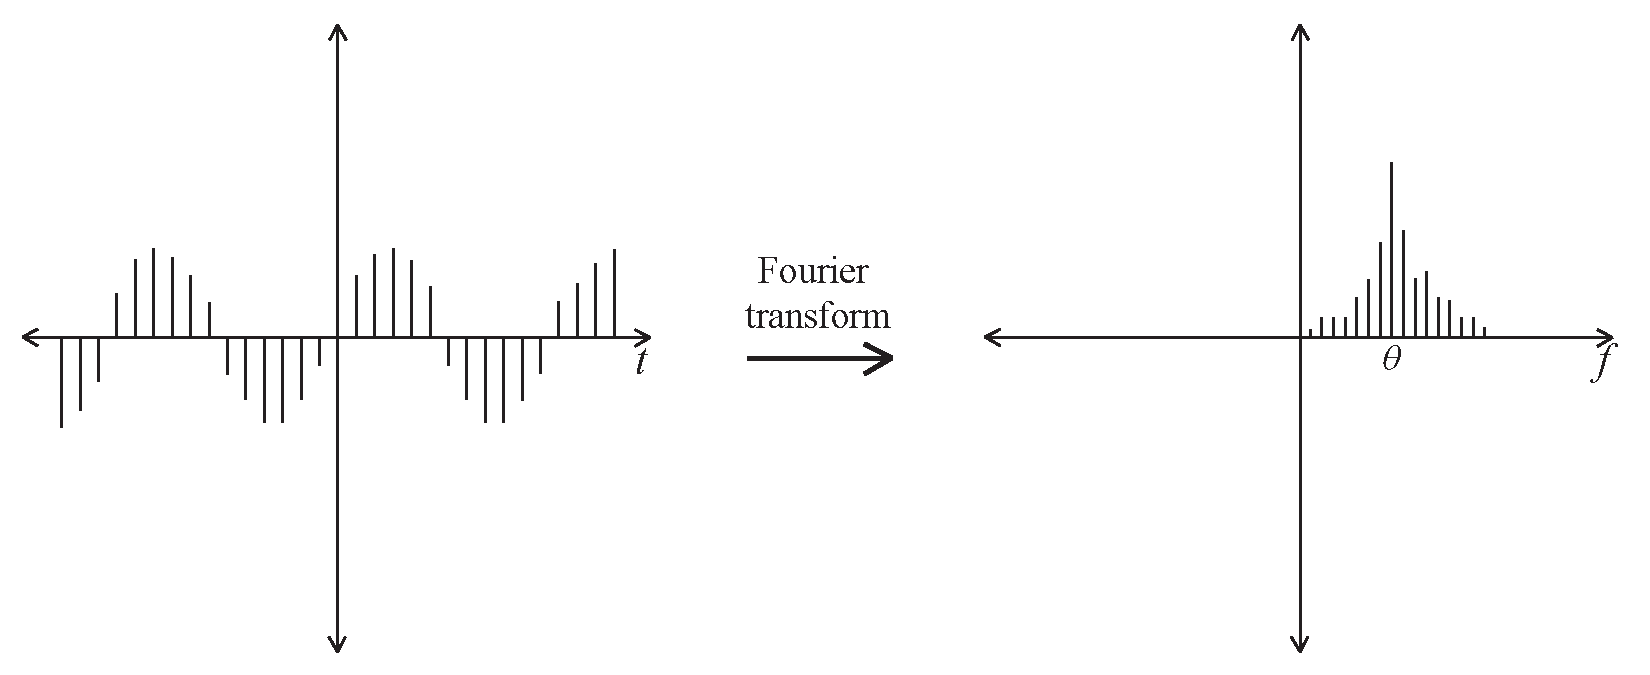
\includegraphics[width=0.8\textwidth]{DFT.pdf}
\caption{The Fourier transform of discrete samples approximating a sine wave with frequency $\theta$ in the time domain results in a rough distribution in the frequency domain peaked at (or near) $\theta$.}
\label{fig:dft}
\end{figure}
As you can see, the frequency decomposition is not as well-defined in the discrete case.
This lack of definition is due to the fact that the information given is incomplete and noisy (error prone).
If you were to increase the number of samples taken, the frequency decomposition would expectedly become cleaner.
However, taking more samples has a drawback in that it takes longer to collect and process them.
The continuous case is basically the result of extending this thought and taking an infinite amount of samples.
Since we can't take an infinite amount of samples, we will just have to settle with the rough peak in the discrete transform.

In Java, the \ac{fft} is implemented as a \verb=static= function of the {\tt FastFourierTransform} class.
It takes an array of \verb=Complex= objects as input, and places its output into the given array.
This means that once you give it something, the input is lost (unless you want to implement the Inverse \ac{fft}).

The \verb=Complex= objects the \ac{fft} takes as arguments are simply representations of complex numbers $a+bi$, where $a$ is the real part and $b$ is the imaginary part.
Complex numbers are intimately related to waves and the \ac{fft}, but the only extent to which you need to understand them is very basic.
As long as you can perform the operations of complex addition, subtraction, multiplication, and division, you should be fine.
The \verb=FastFourierTransform= and \verb=Complex= classes are provided for you in the package {\tt csc120.lab6.FFT}.